% Options for packages loaded elsewhere
\PassOptionsToPackage{unicode}{hyperref}
\PassOptionsToPackage{hyphens}{url}
%
\documentclass[
]{article}
\usepackage{amsmath,amssymb}
\usepackage{lmodern}
\usepackage{iftex}
\ifPDFTeX
  \usepackage[T1]{fontenc}
  \usepackage[utf8]{inputenc}
  \usepackage{textcomp} % provide euro and other symbols
\else % if luatex or xetex
  \usepackage{unicode-math}
  \defaultfontfeatures{Scale=MatchLowercase}
  \defaultfontfeatures[\rmfamily]{Ligatures=TeX,Scale=1}
\fi
% Use upquote if available, for straight quotes in verbatim environments
\IfFileExists{upquote.sty}{\usepackage{upquote}}{}
\IfFileExists{microtype.sty}{% use microtype if available
  \usepackage[]{microtype}
  \UseMicrotypeSet[protrusion]{basicmath} % disable protrusion for tt fonts
}{}
\makeatletter
\@ifundefined{KOMAClassName}{% if non-KOMA class
  \IfFileExists{parskip.sty}{%
    \usepackage{parskip}
  }{% else
    \setlength{\parindent}{0pt}
    \setlength{\parskip}{6pt plus 2pt minus 1pt}}
}{% if KOMA class
  \KOMAoptions{parskip=half}}
\makeatother
\usepackage{xcolor}
\usepackage[margin=1in]{geometry}
\usepackage{longtable,booktabs,array}
\usepackage{calc} % for calculating minipage widths
% Correct order of tables after \paragraph or \subparagraph
\usepackage{etoolbox}
\makeatletter
\patchcmd\longtable{\par}{\if@noskipsec\mbox{}\fi\par}{}{}
\makeatother
% Allow footnotes in longtable head/foot
\IfFileExists{footnotehyper.sty}{\usepackage{footnotehyper}}{\usepackage{footnote}}
\makesavenoteenv{longtable}
\usepackage{graphicx}
\makeatletter
\def\maxwidth{\ifdim\Gin@nat@width>\linewidth\linewidth\else\Gin@nat@width\fi}
\def\maxheight{\ifdim\Gin@nat@height>\textheight\textheight\else\Gin@nat@height\fi}
\makeatother
% Scale images if necessary, so that they will not overflow the page
% margins by default, and it is still possible to overwrite the defaults
% using explicit options in \includegraphics[width, height, ...]{}
\setkeys{Gin}{width=\maxwidth,height=\maxheight,keepaspectratio}
% Set default figure placement to htbp
\makeatletter
\def\fps@figure{htbp}
\makeatother
\setlength{\emergencystretch}{3em} % prevent overfull lines
\providecommand{\tightlist}{%
  \setlength{\itemsep}{0pt}\setlength{\parskip}{0pt}}
\setcounter{secnumdepth}{-\maxdimen} % remove section numbering
\ifLuaTeX
  \usepackage{selnolig}  % disable illegal ligatures
\fi
\IfFileExists{bookmark.sty}{\usepackage{bookmark}}{\usepackage{hyperref}}
\IfFileExists{xurl.sty}{\usepackage{xurl}}{} % add URL line breaks if available
\urlstyle{same} % disable monospaced font for URLs
\hypersetup{
  pdftitle={DROUGHT CONDITIONS IN THE US AND CRITIQUE},
  pdfauthor={JABEN PETER D. BAKO (21322100)},
  hidelinks,
  pdfcreator={LaTeX via pandoc}}

\title{DROUGHT CONDITIONS IN THE US AND CRITIQUE}
\author{JABEN PETER D. BAKO (21322100)}
\date{2023-02-21}

\begin{document}
\maketitle

{
\setcounter{tocdepth}{2}
\tableofcontents
}
GitHub repository: \url{https://github.com/Jabendah/C7083}

\newpage

\hypertarget{drought-conditions-in-the-us}{%
\section{DROUGHT CONDITIONS IN THE
US}\label{drought-conditions-in-the-us}}

\hypertarget{data-background}{%
\section{Data background}\label{data-background}}

The US drought dataset used in this portfolio comes from the the
TidyTuesday Github repo and represents data collected from the National
Integrated Drought Information System dated from 1895 to 2022. The
dataset has information including Date, Five (5) different levels of
drought (Abnormal, Moderate, Severe, Extreme and Exceptional drought),
Five different levels of wetness (Abnormal, Moderate, Severe, Extreme
and Exceptional wet) and State of the United State. This data
information is used in this portfolio to make six (6) different
visualization. More detail about the dataset can be found on the Github
link
\href{https://github.com/rfordatascience/tidytuesday/tree/master/data/2022/2022-06-14}{TidyTuesday}.

\begin{longtable}[]{@{}lll@{}}
\toprule()
Variable & Class & Description \\
\midrule()
\endhead
0 & numeric & Percentage area with no drought \\
DATE & date & Date \\
D0 & numeric & Percentage area with Abnormal Drought \\
D1 & numeric & Percentage area with Moderately Drought \\
D2 & numeric & Percentage area with severe drought \\
D3 & numeric & Percentage area with Extreme Drought \\
D4 & numeric & Percentage area with Exceptional Drought \\
-9 & numeric & Percentage area with missing data \\
W0 & numeric & Percentage area with Abnormal Wet conditions \\
W1 & numeric & Percentage area with Moderate Wet conditions \\
W2 & numeric & Percentage area with Severe Wet conditions \\
W3 & numeric & Percentage area with Extreme Wet conditions \\
W4 & numeric & Percentage area with Exceptional Wet conditions \\
state & character & State \\
\bottomrule()
\end{longtable}

The drought dataset has 14 variables and 73,344 observations from year
1895 to 2022 and 48 States in US.

\newpage

\hypertarget{the-relationship-between-abnormal-drought-and-abnormal-wet-using-base-r}{%
\section{The relationship between Abnormal drought and Abnormal wet
using Base
R}\label{the-relationship-between-abnormal-drought-and-abnormal-wet-using-base-r}}

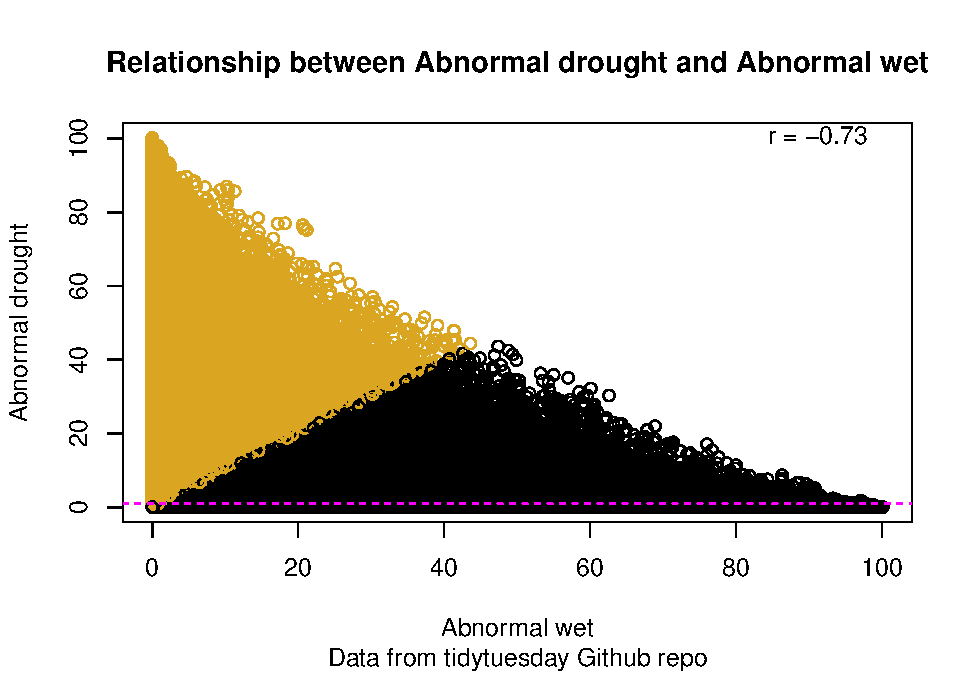
\includegraphics{C7083-213221-Markdown_files/figure-latex/Scatter plot of Abnormal drought and Abnormal wet-1.pdf}
Figure 1: Scatter plot of the Relationship between Abnormal Drought and
Abnormal Wet

Figure 1 shows a negative relationship between abnormal drought and
abnormal wet condition of -0.73 correlation coefficient and a line to
the plot using the abline function. This line has an intercept of 1 and
a slope of 0, and it is drawn with a dashed line type (lty = 2) and a
magenta color (col = ``magenta''). The correlation coefficient value to
the plot using the text function. The text is placed at the top right
corner of the plot (pos = 2), and its x and y coordinates are set to the
maximum values of abnormal drought and abnormal wet conditions,
respectively.

\hypertarget{bar-chart-of-drought-severity-by-state-using-ggplot}{%
\section{Bar Chart of drought severity by state using
ggplot}\label{bar-chart-of-drought-severity-by-state-using-ggplot}}

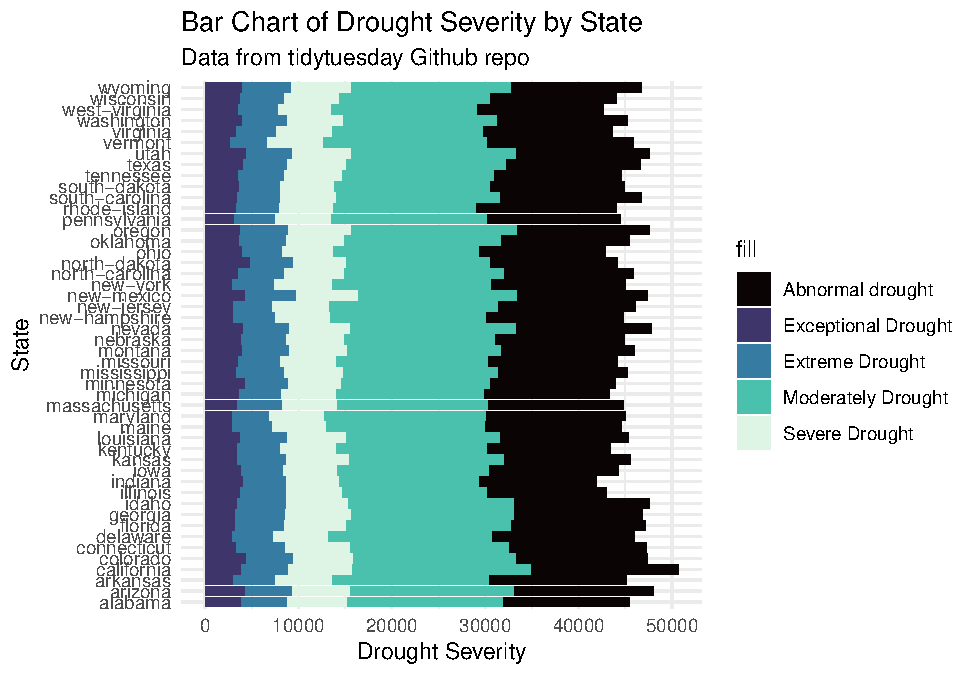
\includegraphics{C7083-213221-Markdown_files/figure-latex/Bar Chart of drought severity-1.pdf}
Figure 2: Bar chart of Drought levels by States

Figure 2 used the aesthetic function in ggplot to map the drought level
plot. The x aesthetic is set to the State variable, and y is set to the
severity of Abnormal, Moderate, Sever, Extreme, and Exceptional drought.
The geom\_bar function is used to create the bars for each drought
level, and the fill aesthetic is set to the severity level name and it
is observed that Moderate drought has the highest severity across the
states. The coord\_flip function was used to flip the chart horizontally
to make it easier to read the state names.

\hypertarget{drought-severity-levels-over-time-from-2000-to-2022-using-line-plot}{%
\section{Drought Severity levels over time from 2000 to 2022 Using line
plot}\label{drought-severity-levels-over-time-from-2000-to-2022-using-line-plot}}

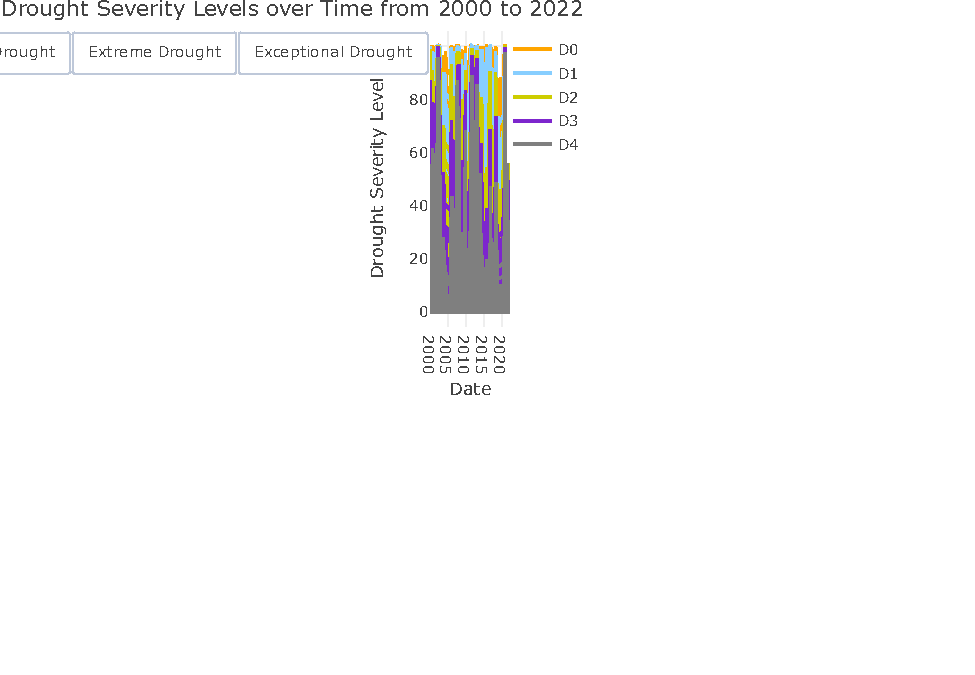
\includegraphics{C7083-213221-Markdown_files/figure-latex/Interactive line plot for drought severity levels over time-1.pdf}
Figure 3: Interactive line plot for drought severity levels over time.

The above plot in figure 3 shows a line plot with a drop-down menu to
select different drought severity levels over time. It shows the trends
and changes in drought severity levels from 2000 to 2022 with the help
of the function plotly. From the visualization, Abnormal drought has
more residuals and Exceptional drought has the the least when clicked
through the selected years.

\hypertarget{combination-of-a-line-chart-and-a-scatter-plot-with-jittered-points-of-abnormal-drought-conditions-over-time-ggplot}{%
\section{Combination of a line chart and a scatter plot with jittered
points of Abnormal drought conditions over time
(ggplot)}\label{combination-of-a-line-chart-and-a-scatter-plot-with-jittered-points-of-abnormal-drought-conditions-over-time-ggplot}}

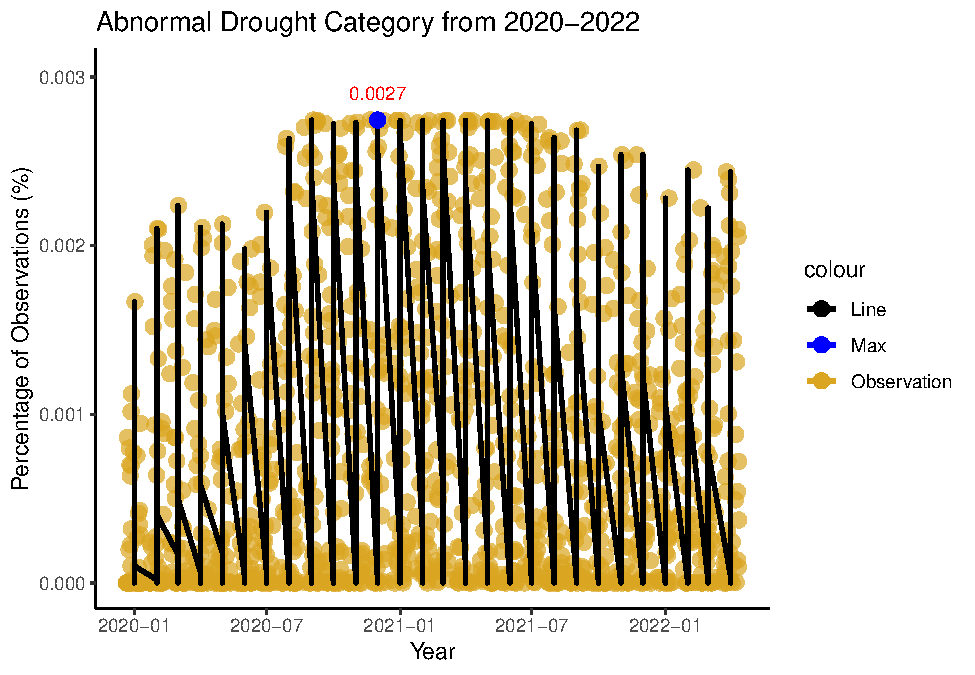
\includegraphics{C7083-213221-Markdown_files/figure-latex/line plot with jittered points-1.pdf}
Figure 4: Percentage of observations in the Abnormal Drought Category
from 2020 to 2022

Figure 4 shows the percentage observation of abnormal drought from year
2000 - 2022 which visualizes the maximum value and its corresponding
date in the data, rounds the maximum value to 4 decimal places, and then
uses ggplot to create a jittered line chart and with the maximum value
point of 0.0027 within the last part of year 2020 and its label
highlighted in blue. The plot is customized with axis labels, title,
theme, and color scheme.

\hypertarget{time-series-plot-of-drought-and-wet-conditions-over-time-ggplot}{%
\section{Time series plot of drought and wet conditions over time
(ggplot)}\label{time-series-plot-of-drought-and-wet-conditions-over-time-ggplot}}

\begin{verbatim}
## 
## Listening on http://127.0.0.1:7960
\end{verbatim}

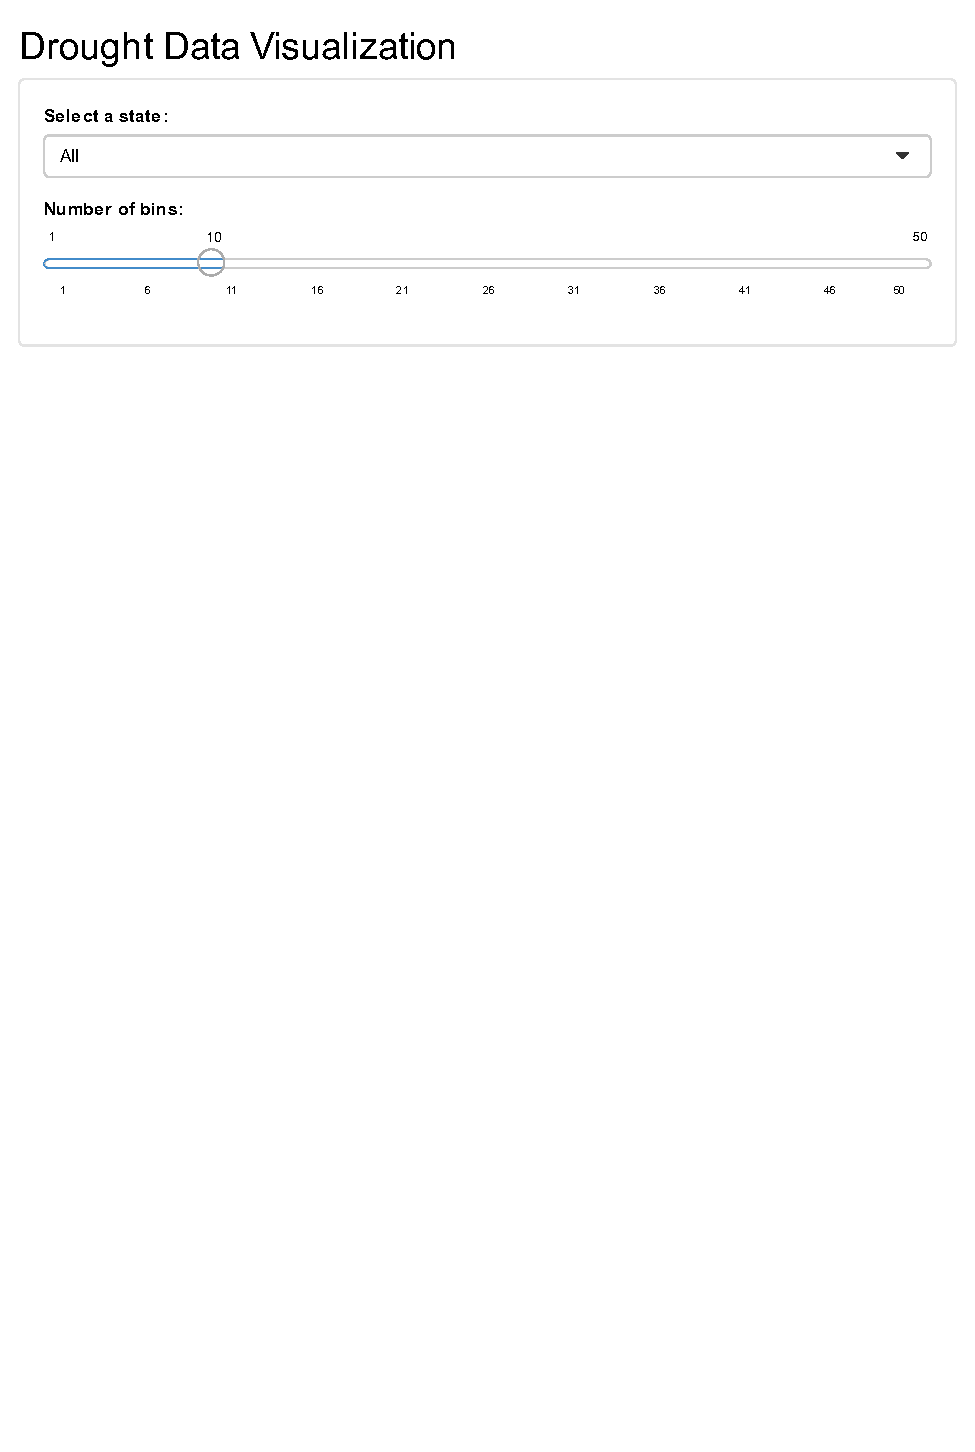
\includegraphics{C7083-213221-Markdown_files/figure-latex/Interactive plot of drought with state-1.pdf}

\begin{figure}
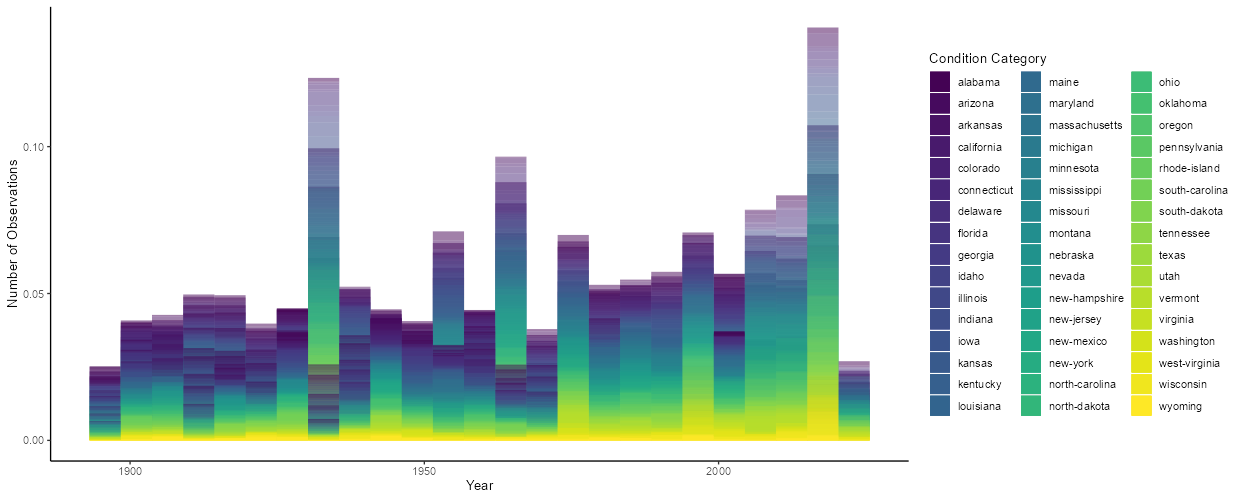
\includegraphics[width=1\linewidth]{../Images/Drought_Shiny} \caption{Drought with State over time}\label{fig:Figure 5-1}
\end{figure}

Figure 5: Interactive plot of drought with state data over time using
Shiny

The output of figure 5 was created using Shiny app for visualizing
drought data. The app has a sidebar panel with input controls for
selecting a state and the number of bins in the histogram. The main
panel displays a histogram plot that shows the percentage of
observations in each condition category for the selected state. The
visualization filters the data based on the selected state and
calculates the percentage of observations in each category. The
histogram is created using ggplot and has a legend that shows the fill
color for each condition category. The app can be viewed on shiny. with
the drop-down one can choose to view individual state or All the state
to see their drought level.

\hypertarget{interactive-map-of-us-showing-the-total-drought-sum}{%
\section{Interactive map of US showing the total drought
sum}\label{interactive-map-of-us-showing-the-total-drought-sum}}

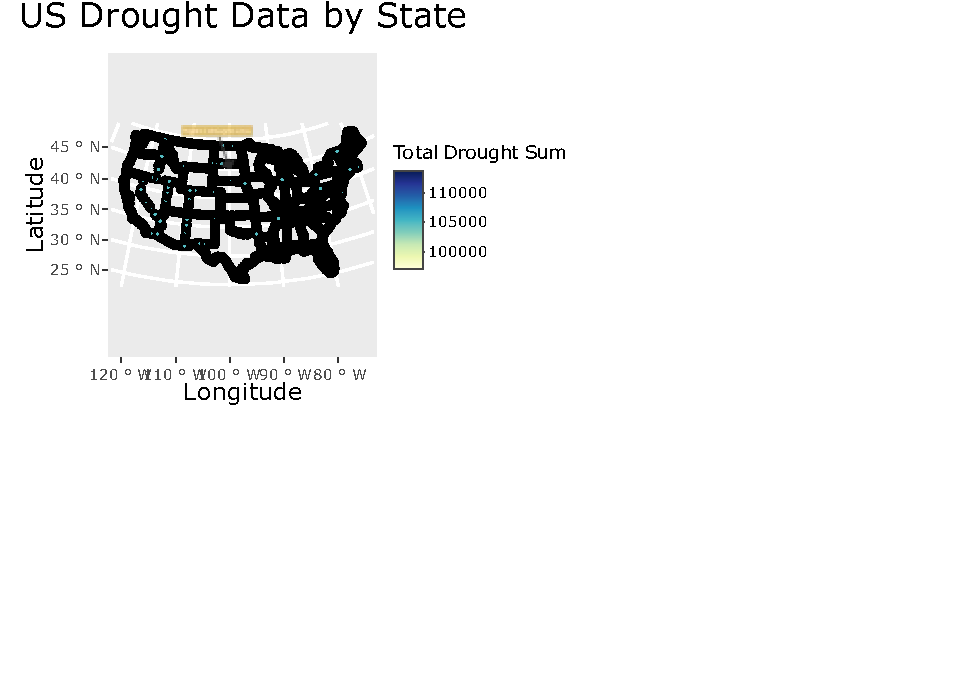
\includegraphics{C7083-213221-Markdown_files/figure-latex/Interactive map of US-1.pdf}
Figure 6:Interactive map of US showing the total drought sum

Figure 6 shows US state data on drought, aggregates of the drought data
by state, joins of the aggregated data with state data, and plot of the
total drought severity by state using ggplot2 and plotly. The resulting
plot shows an interactive map of the US with states colored by the
severity of drought. As the mouse moves over and through the map, total
drought of the state is displayed and an arrow showing the area with the
highest number of droughts around South Dakota.

\newpage

\hypertarget{critique}{%
\section{CRITIQUE}\label{critique}}

\hypertarget{good-visualization}{%
\section{Good Visualization}\label{good-visualization}}

\begin{figure}
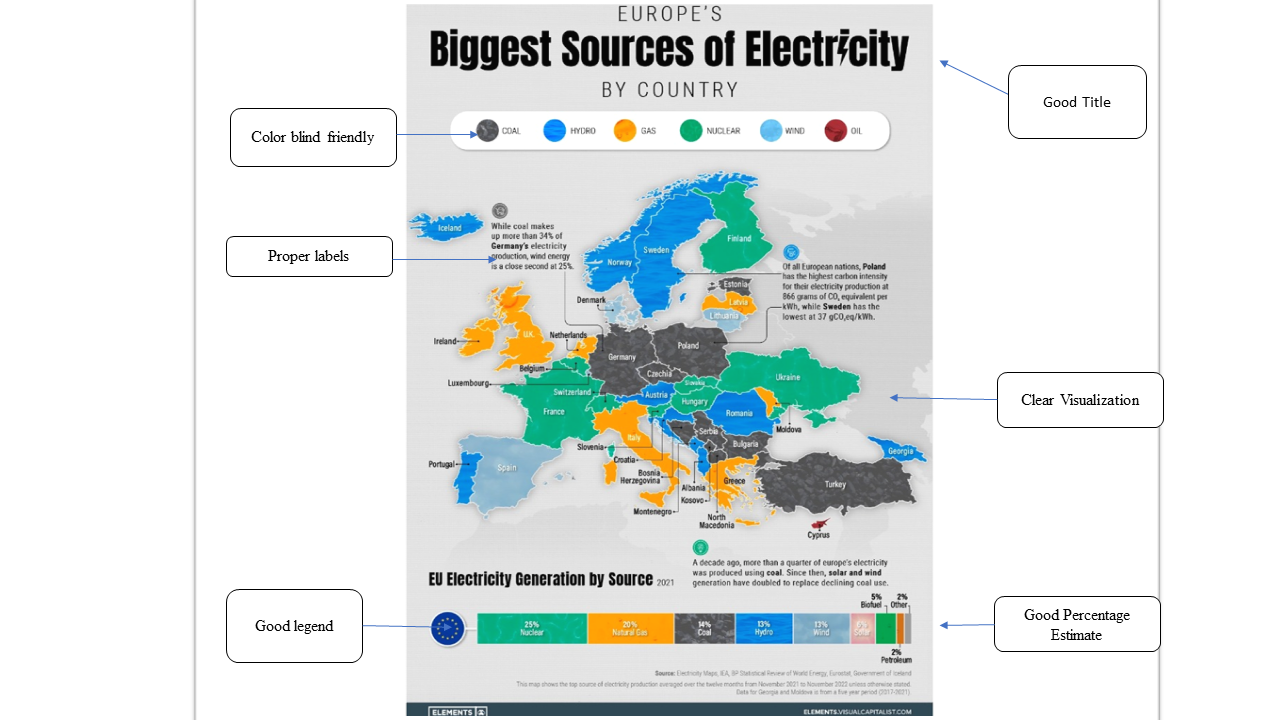
\includegraphics[width=1\linewidth]{../Images/Good Vis} \caption{Europe's Biggest Source of Electricity}\label{fig:Good Visualization}
\end{figure}

The visualization in Figure 7 provides a clear and concise overview of
Europe's biggest sources of electricity by country. The map is an
effective tool for communicating complex information to a wide audience,
as it is easy to read, understand, and interpret. The map's title is
descriptive, and it provides readers with a clear understanding of what
they will be viewing. The color scheme is distinctive, making it easy
for readers, including color-blind readers, to differentiate between
energy sources. The placement of the legends and labels is appropriate,
with areas of interest clearly labeled and statistical percentages
accurately recorded. The clarity of the visualization ensures that
readers can easily navigate the map without any help. Additionally, the
labeled countries make it easy for those without a strong background in
geography to understand which countries are being represented. The
visualization's purpose is clearly conveyed, as readers can easily
understand the distribution of electricity sources across Europe. The
map allows readers to quickly identify the countries that rely heavily
on certain sources of energy, providing valuable insights into the
energy landscape of Europe. In conclusion, the visualization in Figure 7
is an effective communication tool that provides readers with a clear
and concise overview of Europe's biggest sources of electricity by
country. The map's well-designed title, distinctive color scheme,
appropriate labels, and accurate statistics make it easy for readers to
read, understand, and interpret the information presented. Overall, the
visualization meets its purpose of informing readers about Europe's
energy sources while also being accessible to a wide audience.

\newpage

\hypertarget{bad-visualization}{%
\section{Bad Visualization}\label{bad-visualization}}

\begin{figure}
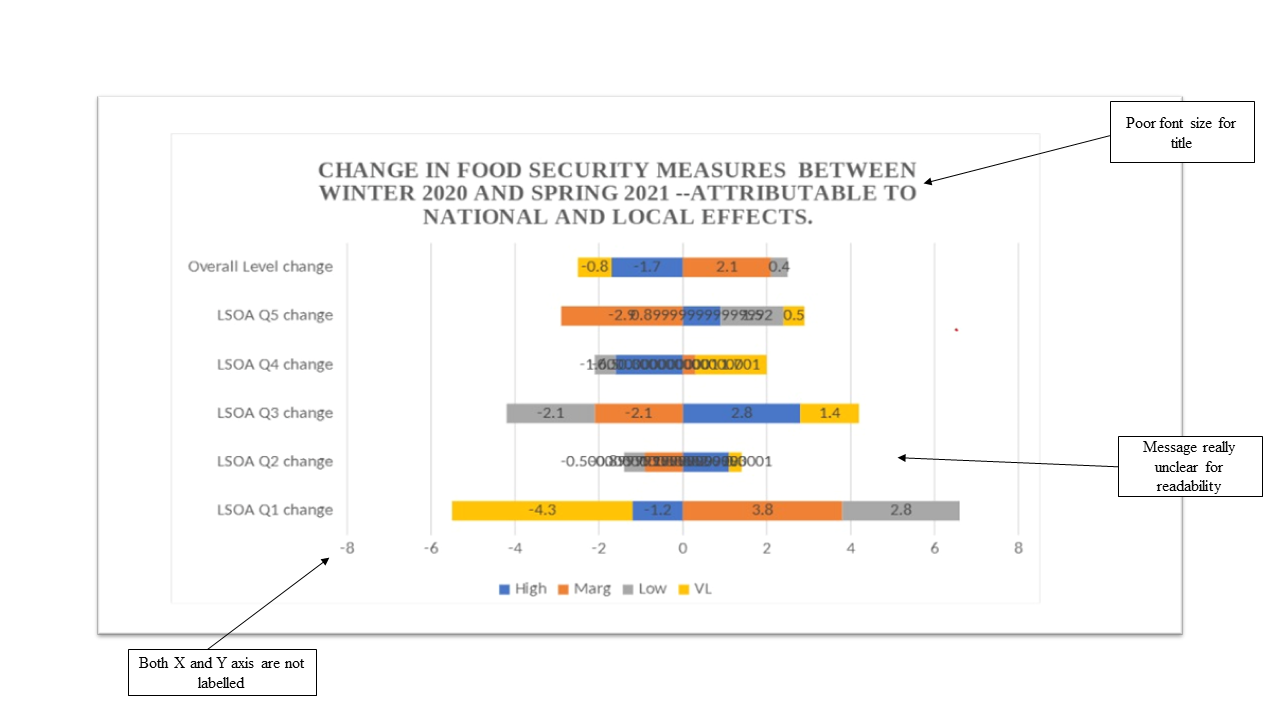
\includegraphics[width=1\linewidth]{../Images/Bad Viz} \caption{Changes in Food Security Measures}\label{fig:Bad Visualization}
\end{figure}

Figure 8 displays a bar graph that aims to illustrate the changes in
food security measures between Winter 2002 and Spring 2021 and the
contribution of both national and local effects. Although the
visualization has a title, the font size is too big and may distract the
reader from the actual message. Furthermore, the lack of labels for both
the X and Y axes makes it difficult for the reader to comprehend what
each outlined point or variable represents.

The message that was intended to be conveyed in the graph is unclear due
to the poor spacing of figures in the bars. It is challenging to read
the plot without serious mental calculations and straining of the eyes.
Without a good knowledge of the subject topic, it is almost impossible
for anyone to understand the changes within the plot and what each value
represents.

One way to improve the visualization is by labeling the axes. This will
make it easier for the reader to understand what each variable
represents. Additionally, keeping the graph simple by making space to
expand the graphics will enhance readability. Moreover, the audience
should be the focus of the presentation, and this will influence the
choice of graph. It may be more effective to use a line graph, which can
better illustrate changes over time.

In conclusion, Figure 8's bar graph fails to communicate the intended
message due to the lack of axis labels, poor spacing, and excessive font
size. By implementing the proposed changes, such as labeling the axes
and using a simpler, more reader-friendly graph type, the visualization
could be more effective in conveying its message. The changes will
enhance the visualization's readability, making it easier for readers to
understand the changes in food security measures between Winter 2002 and
Spring 2021.

\newpage

\hypertarget{reference}{%
\section{Reference}\label{reference}}

Dr Joe Roberts. (2022). Online resources on the learning hub. Retrieved
from \url{https://hub.harperadams.ac.uk/course/view.php?id=5832}

Megan, B., \& Jonas, C. (2022). Food Insecurity within UK Communities.
{[}Online{]}. Retrieved from
\url{https://www.researchgate.net/publication/365362129_Food_Security_UK_2021?channel=doi\&linkId=6372231a37878b3e87aea86c\&showFulltext=true\#fullTextFileContent}

Plotly. (2023). Online examples. Retrieved from
\url{https://plotly.com/examples/}

Unwin, A. (2020). Why is Data Visualization Important? What is Important
in Data Visualization? Harvard Data Science Review, 2(1).
\url{https://doi.org/10.1162/99608f92.8ae4d525}

VisualCapitalist. (2019). Europe's Biggest Sources of Electricity by
Country. {[}Online{]}. Retrieved from
\url{https://www.visualcapitalist.com/mapped-europes-biggest-sources-of-electricity-by-country/}

\end{document}
